\section{The model}
\subsection{Introduction}

\begin{frame}
  \frametitle{What is unsupervised learning?}
  \emph{Unsupervised learning} is a class of algorithms that learn patterns from \alert{uncategorized data}. \\
  The model works on its own to discover representation previously undetected. \\
  \vspace{15pt}
  We would like to learn the \alert{probability distribution} of a \emph{training set}.
  \pause
  \begin{alertblock}{Example: handwritten digits}
    We would like our model to learn that a given handwritten digit (not necessarily belonging to the training set) has a higher probability
    than a generic image. We want to achieve this by training the model with some handwritten digits, without telling it which number the image contains.
  \end{alertblock}
\end{frame}

\subsection{RBM basic properties}
\begin{frame}
  \frametitle{What is a Restricted Boltzmann Machine?}
  \begin{itemize}
    \item<1-> Two sets of \alert{units}
      \begin{itemize}
        \item \structure{visible layer}: \(\mathcal{V} = \{V_1, \dots, V_m\}\) are features of the empirical distribution
        \item \structure{hidden layer}: \(\mathcal{H} = \{H_1, \dots, H_n\}\) are only used internally by the machine
      \end{itemize}
    \item<2-> The units are \alert{binary}: \(v_i, h_j \in \{0,1\}\)
    \item<3-> The \alert{Markov Property} applies
      \begin{align*}
        \CondProb{V_i}{\{V_{i'}\}_{V_{i'}\in (\mathcal{V} \setminus \{V_i\})}, \{H_j\}_{H_j\in \mathcal{H}}} =
        \CondProb{V_i}{\{H_j\}_{H_j\in \mathcal{H}}} \\
        \CondProb{H_j}{\{V_i\}_{V_i\in \mathcal{V}}, \{H_{j'}\}_{H_{j'}\in (\mathcal{H} \setminus \{H_j\})}} =
        \CondProb{H_j}{\{V_i\}_{V_i\in \mathcal{V}}}
      \end{align*}
  \end{itemize}
	\begin{figure}[<1->]
		\resizebox{0.6\textwidth}{!}{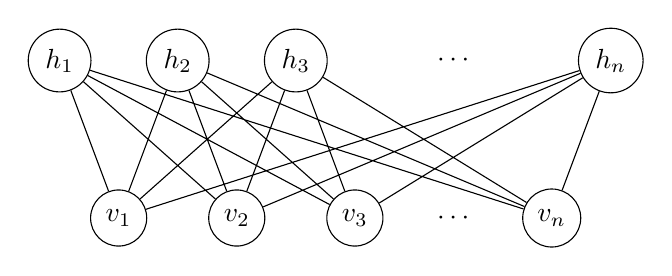
\begin{tikzpicture}%[node distance={15mm}, thick, main/.style = {draw, circle}] 
  \node[draw, circle] (h1) at (1.5,1)   {$h_1$}; 
  \node[draw, circle] (h2) at (3,1)   {$h_2$};
  \node[draw, circle] (h3) at (4.5,1)   {$h_3$};
  \node            (hdots) at (6.5,1) {$\cdots$};
  \node[draw, circle] (hn) at (8.5,1)   {$h_n$};
  
  \node[draw, circle] (v1) at (2.25,-1)   {$v_1$}; 
  \node[draw, circle] (v2) at (3.75,-1)   {$v_2$};
  \node[draw, circle] (v3) at (5.25,-1)   {$v_3$};
  \node            (vdots) at (6.5,-1) {$\cdots$};
  \node[draw, circle] (vm) at (7.75,-1)   {$v_n$};
  
  \draw (v1)--(h1)
        (v1)--(h2)
        (v1)--(h3)
        (v1)--(hn)
        (v2)--(h1)
        (v2)--(h2)
        (v2)--(h3)
        (v2)--(hn)
        (v3)--(h1)
        (v3)--(h2)
        (v3)--(h3)
        (v3)--(hn)
        (vm)--(h1)
        (vm)--(h2)
        (vm)--(h3)
        (vm)--(hn);
\end{tikzpicture} }
	\end{figure}
\end{frame}

\begin{frame}
  \frametitle{Probability distribution}
	It can be proven that
	\[\prob{\vec{v}, \vec{h}} = \frac{1}{Z} \exp\left(-E(\vec{v}, \vec{h})\right)
	\quad\text{ where }\quad
	Z = \sum_{\vec{v}, \vec{h}}\exp\left(-E(\vec{v}, \vec{h})\right)\]
	\pause
	Allowing only polynomial energy:
	\[
	E(\vec{v}, \vec{h}) = -\sum_{i}^m b_i v_i - \sum_{j}^n c_j h_j -
	\sum_{i=1,j=1}^{m,n} v_i w_{i,j} h_j
	\]
  \pause
  This is an \alert{Ising Model}:
  \begin{itemize}
    \item \(\beta = 1\)
    \item \(b_i, c_j\) are local fields
    \item \(w_{i,j}\) are intra-layer interactions
  \end{itemize}
\end{frame}

\begin{frame}
  \frametitle{Some other properties}
  \begin{itemize}
    \item<1-> The Markov property implies
      \[
        \condprob{\vec{h}}{\vec{v}} = \prod_{j=1}^n \condprob{h_j}{\vec{v}} \quad\text{and}\quad
        \condprob{\vec{v}}{\vec{h}} = \prod_{i=1}^m \condprob{v_i}{\vec{h}}.
      \]
    \item<2-> Conditional activation probabilities can be computed analytically:
      \begin{align*}
        \condprob{h_j=1}{\vec{v}} &= \sigmoid{\sum_{i=1}^m w_{i,j}v_i+c_j},\\
        \condprob{v_i=1}{\vec{h}} &= \sigmoid{\sum_{j=1}^n w_{i,j}h_j+b_i}.
      \end{align*}
      where \(\sigmoid{\cdot}\) is the \alert{logistic function} \(\frac{1}{1+e^{-x}}\).
  \end{itemize}
\end{frame}

%%%%%%%%%%%%%%%%%%%%%%%%%%%%%%%%%%%%%%%%%%%%%%%%%%%%%%%%%%%%%%%%%%%%%%%%%%%%%%%%%%%%%%%%%%%%%%%%%%%%

\subsection{Likelihood Maximization}
\begin{frame}
\frametitle{Likelihood}
  \begin{itemize}
		\item The basic idea of all training algorithms is \alert{to~maximize~the~(log)likelihhod}
		\item \(S = \left\{\vec{\bar{v}}_k\right\}_{k \in \{1,\dots,\ell\}}\) is the training set;\\
      \(\vec{\theta}\) is the set of model parameters
		  \[
			 \log\likelihood{\vec{\theta}}{S} = \sum_{k=1}^\ell \log\left(\prob{\vec{\bar{v}}_k;\vec{\theta}}\right)
		  \]
		\pause
    \item \alert{Gradient ascent} is used. The likelihood gradient is
      \[
         \ParDer{\log\likelihood{\vec{\theta}}{\vec{\bar{v}}}}{\vec{\theta}} =
         	\underbrace{-\ExpVal{\condprob{\vec{h}}{\vec{\bar{v}}}}{\ParDer{E(\vec{\bar{v}},\vec{h})}{\vec{\theta}}}}_{\text{comes from } e^{-E(\vec{\bar{v}},\vec{h})}}
          +\underbrace{\ExpVal{\prob{\vec{v},\vec{h}}}{\ParDer{E(\vec{v},\vec{h})}{\vec{\theta}}}}_{\text{comes from } Z}
      \]
	\end{itemize}
\end{frame}

\begin{frame}
  \frametitle{Bernoulli RBM likelihood gradient}
  \begin{align*}
    % gradient of w_{i,j}
    \ParDer{\log\likelihood{\vec{\theta}}{\vec{\bar{v}}}}{w_{i,j}}
    &= \bar{v}_i \sigmoid{\sum_{i'=1}^m w_{i',j}\bar{v}_{i'}+c_j}
    -\ExpVal{\prob{\vec{v}}}{v_i \sigmoid{\sum_{i=1}^m w_{i',j}v_{i'}+c_j}} \\[5pt]
    % gradient of b_i
    \ParDer{\log\likelihood{\vec{\theta}}{\vec{\bar{v}}}}{b_i}
    &= \bar{v}_i -\ExpVal{\prob{\vec{v}}}{v_i} \\[5pt]
    % gradient of c_j
    \ParDer{\log\likelihood{\vec{\theta}}{\vec{\bar{v}}}}{c_j}
    &= \sigmoid{\sum_{i=1}^m w_{i',j}\bar{v}_{i'}+c_j}
    -\ExpVal{\prob{\vec{v}}}{\sigmoid{\sum_{i=1}^m w_{i',j}v_{i'}+c_j}}
  \end{align*}
	\visible<2->{
		\begin{columns}
			\column{0.75\textwidth}
	  	\begin{alertblock}{Problem!}
	    	These expected values are uncomputable in practice! \(\#\{\vec{v}\} = 2^m\).
	  	\end{alertblock}
  	\end{columns}
  }
\end{frame}



